\documentclass[11pt]{article}
\usepackage{amsmath}
\usepackage{graphicx}
\usepackage{hyperref}
\usepackage{tikz}
\usetikzlibrary{positioning}
\usepackage{float}
\usepackage{enumitem}
\usepackage{subcaption}  % for sub-figure environments
\usepackage[margin=1in]{geometry}
\usepackage{listings}
\usepackage{xcolor}

\definecolor{codebg}{rgb}{0,0,0}
\definecolor{codefg}{rgb}{1,1,1}
\definecolor{codegray}{rgb}{0.5,0.5,0.5}

\lstset{
  backgroundcolor=\color{codebg},
  basicstyle=\ttfamily\small\color{codefg},
  frame=single,
  breaklines=true,
  showstringspaces=false,
  tabsize=2,
  captionpos=b,
  numbers=left,
  numberstyle=\tiny\color{codegray},
  xleftmargin=2em,
  xrightmargin=2em
}

\title{\textbf{DSP Worksheet IV}}
\author{Kyle Smith, Ishaan Jagyasi, Peyman Salimi}
\date{28th April 2025}

\begin{document}
\maketitle

\section{Score Sonification}

\subsection{Implementation}

We implemented two types of synthesis techniques, FM and Waveguide synthesis and added a reverb to both the synthesis files using a version of the Schroeder's reverb algorithm. 

\subsection{Documentation of Algorithm}

\subsubsection{MIDI Parsing (same for both the synthesis algorithms)}

We first converted the score to MIDI by writing it in MuseScore and exporting it in MIDI. Then we proceeded to use the `\texttt{pretty\_midi}' library in python to parse the midi file into individual midi note pitches, lengths and velocity. 

We created an empty array to store the output of the synthesis process by finding the total length of the MIDI file. The next step was to iterate through notes and for each note find the start index (in samples), end index, note length (in samples) and total duration of the sample in samples. The total duration of the sample was then used to create a time ramp for each note's duration. 

\begin{lstlisting}[language= Python]
midi_data = pretty_midi.PrettyMIDI(midi_path)
total_duration = midi_data.get_end_time()
audio = np.zeros(int(fs * total_duration))

for instrument in midi_data.instruments:
        for note in instrument.notes:
            start_time = note.start
            end_time = note.end
            duration = end_time - start_time
            start_idx = int(start_time * fs)
            end_idx = int(end_time * fs)
            num_samples = end_idx - start_idx
            t = np.linspace(0, duration, num_samples, endpoint=False)
\end{lstlisting}

After parsing, we carried out synthesis process for each individual note so as to sonify the MIDI file with the chosen synthesis approach. 

\subsubsection{FM Synthesis}

Our approach for FM synthesis was to create a modulator sine wave which in harmonic coherence with the main carrier frequency. To ensure this, we created a variable called `\texttt{harmonic\_ratio}', which defines the relation between the carrier tone frequency to modulator frequency as - 
\begin{equation}
f_m = \text{harmonic\_ratio} \times f_0
\end{equation}

where $f_m$ is the modulator frequency and $f_0$ is the carrier frequency ($f_0$ corresponded to the pitch of the midi note).

Since we created an array for each individual MIDI note, we could store specific carrier wave frequency for each MIDI note and find the harmonically relevant modulator wave frequency. 

The formulae for modulator looked like following:- 

\begin{equation}
    modulator = sin (2\pi f_mt)
\end{equation}

The output of the carrier wave after FM was calculated as follows - 

\begin{equation}
    carrier = sin (2\pi f_0t + I_msin(2 \pi f_mt) )
\end{equation}

We implemented a simple exponential envelope using \texttt{np.exp()}. To make the envelope longer or shorter, we added an option to change the \texttt{decay\_rate} of the exponential envelope. With the envelope implemented, the final output was calculated as follows: 

\begin{lstlisting}[language= Python]
envelope = np.exp(-decay_rate * t)

f0 = pretty_midi.note_number_to_hz(note.pitch)
fm = harmonic_ratio * f0
beta = mod_index

modulator = np.sin(2 * np.pi * fm * t)
carrier = np.sin(2 * np.pi * f0 * t + beta * modulator)

signal = carrier * envelope * (note.velocity / 127.0)
\end{lstlisting}

In order to make the sound more dynamic, we implemented a first-order IIR filter with key tracking to expose more high-frequency content for higher frequency notes. in addition this, we also used the same exponential envelope as the filter envelope. To have extensive control over the cutoff frequency of the filter, we added a \texttt{min\_cutoff} parameter that controls the minimum cutoff frequency and a \texttt{max\_cutoff\_mul} parameter that is a multiplier for $f_0$ to control how much above carrier frequency the filter should open (in order to expose the higher partials created as a result of frequency modulation). 

\begin{lstlisting}[language = Python]
y = np.zeros_like(signal)
y_prev = 0.0
for i in range(len(signal)):
    fc = min_cutoff + envelope[i] * (f0 * max_cutoff_mul - min_cutoff)
    alpha = (2 * np.pi * fc / fs) / (2 * np.pi * fc / fs + 1)
    y[i] = y_prev + alpha * (signal[i] - y_prev)
    y_prev = y[i]
\end{lstlisting}

\begin{figure}[H]
    \centering
    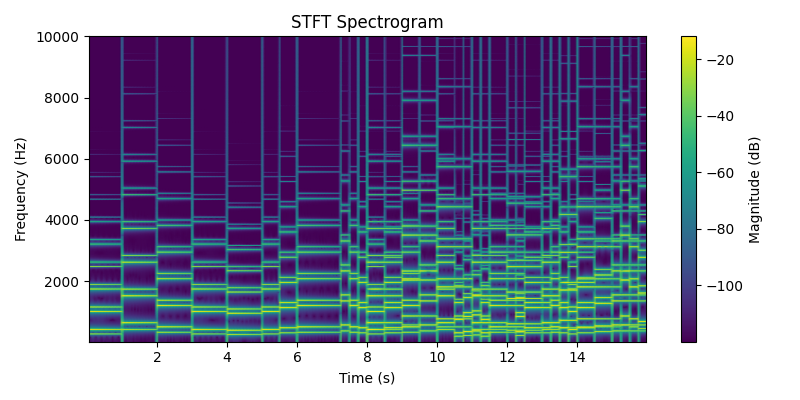
\includegraphics[width=1\textwidth]{FM_synth_Pre_Filter.png}
    \caption{STFT of FM Synthesized Output - Pre Filter} % This is the caption that serves as the image's name
    \label{fig:Fm Synth Out Pre Filter} % This label can be used to reference the image later
\end{figure}

(Figure~\ref{fig:Fm Synth Out Pre Filter}) represents the STFT of the FM synthesized output signal \textbf{pre-filter}. Compared to (Figure~\ref{fig:Fm Synth Out}), which is the output of the FM synthesized signal \textbf{post-filter}, we can see that the filter cuts the higher frequency content in the lower notes, but maintains the high frequency content in the higher notes, which are situated around the 8 second mark in the composition. 

\begin{figure}[H]
    \centering
    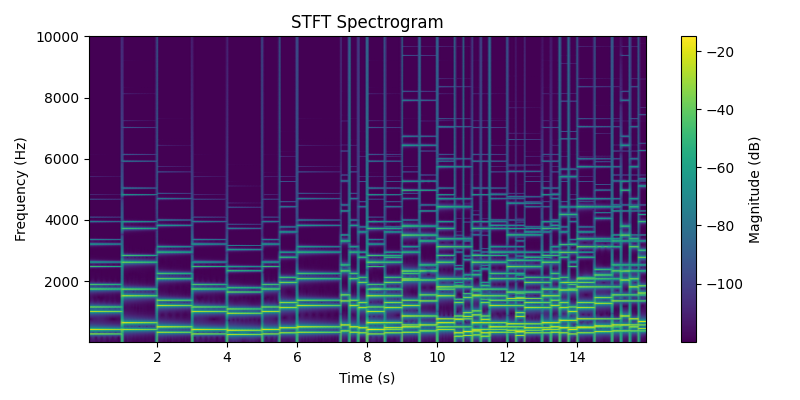
\includegraphics[width=1\textwidth]{FM_Synth_out.png}
    \caption{STFT of FM Synthesized Output - Post Filter} % This is the caption that serves as the image's name
    \label{fig:Fm Synth Out} % This label can be used to reference the image later
\end{figure}

The frequency v.s. magnitude response of the one-pole dynamic filter is represented in (Figure~\ref{fig:Filter Response})

\begin{figure}[H]
    \centering
    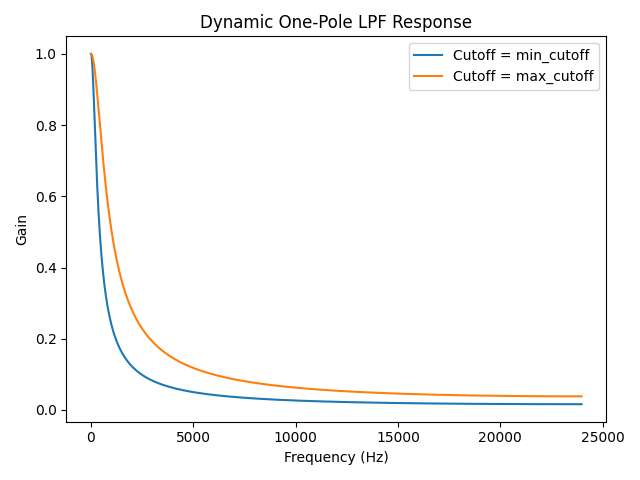
\includegraphics[width=0.7 \textwidth]{Filter_Response_FM.png}
    \caption{Frequency Response of the Dynamic One-Pole Filter} % This is the caption that serves as the image's name
    \label{fig:Filter Response} % This label can be used to reference the image later
\end{figure}

We can also take a look at the frequency content of first notes and is building step. We can see from (Figure~\ref{fig:Car Freq pre}) and (Figure~\ref{fig:Car signal post filt}) that the signal does get affected by the filter (loses frequencies at around 2000 Hz and above) but when we apply the envelope to the filter and the signal, we recover some of that higer frequency content, as shown in (Figure~\ref{fig:Car post fil post env}).

\subsubsection{Waveguide Synthesis}

For waveguide synthesis we defined a class called \texttt{waveGuide} that mimics the movement of a wave on a double bounded string, to and fro from the bridge (left) and the nut (right). We set two delay lines \texttt{x\_L} and \texttt{x\_R} denoting left and right movement of the string along with a loss function \texttt{g()} consisting of a moving average filter at the boundaries. 

The buffer simply moves from left to right through the loss function and that is done through the \texttt{np.roll()} function to push the buffer towards the right every sample. 

The excitation function used in this case is a simple triangular pluck function with maximum y-directional displacement at a place that can be defined while calling the synthesis function. 

To synthesize the audio, we defined a \texttt{synthesize\_midi()} function that takes in the MIDI file to be synthesized, relative position of the pluck and pickup position (in fraction of the length of the buffer).

The base frequency of each note (extracted from \texttt{pretty\_midi} is used to define the buffer size by the formula 
\begin{equation}
    L = f_s/2f    
\end{equation}


where $f$ is the pitch of each note and $f_s$ is the sampling rate. Since $1/f$ would define the time period of this frequency, we can multiply it by the sampling rate and double it to get the total number of samples required for the left plus right traveling buffers. 




\begin{figure}[H]
    \centering
    \begin{subfigure}[b]{0.45\textwidth}
        \centering
        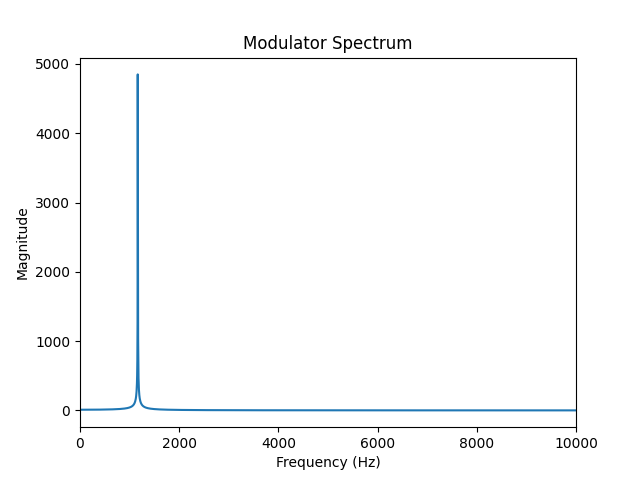
\includegraphics[width=\textwidth]{Modulator Spectrum.png}
        \caption{Frequency Spectrum of Modulator Signal}
        \label{fig:Mod Sign Freq Spec}
    \end{subfigure}
    \hfill
    \begin{subfigure}[b]{0.45\textwidth}
        \centering
        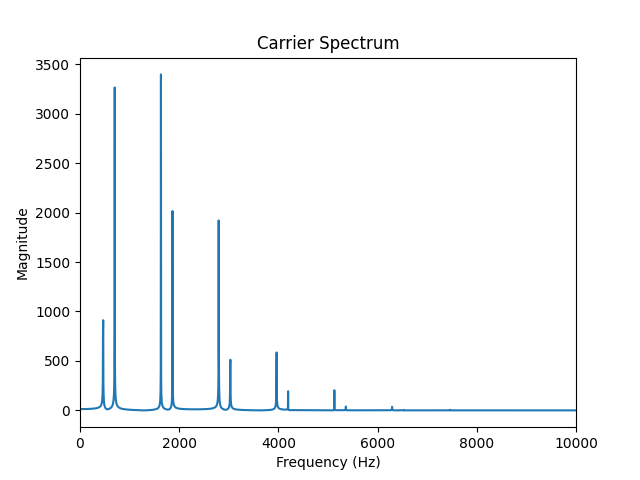
\includegraphics[width=\textwidth]{Carrier Spectrum(noenv and Filter).png}
        \caption{Carrier Signal Frequency Spectrum Pre-Filter and Pre-Envelope}
        \label{fig:Car Freq pre}
    \end{subfigure}
    \vskip\baselineskip
    \begin{subfigure}[b]{0.45\textwidth}
        \centering
        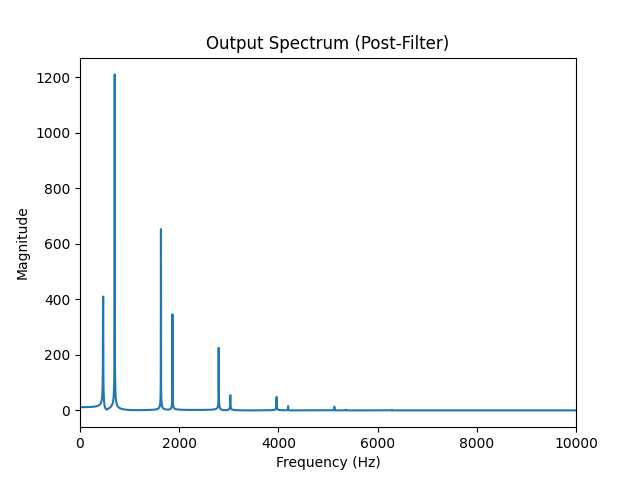
\includegraphics[width=\textwidth]{Carrier Signal Post Filter.png}
        \caption{Carrier Signal Frequency Spectrum Post-Filter and Pre-Envelope}
        \label{fig:Car signal post filt}
    \end{subfigure}
    \hfill
    \begin{subfigure}[b]{0.45\textwidth}
        \centering
        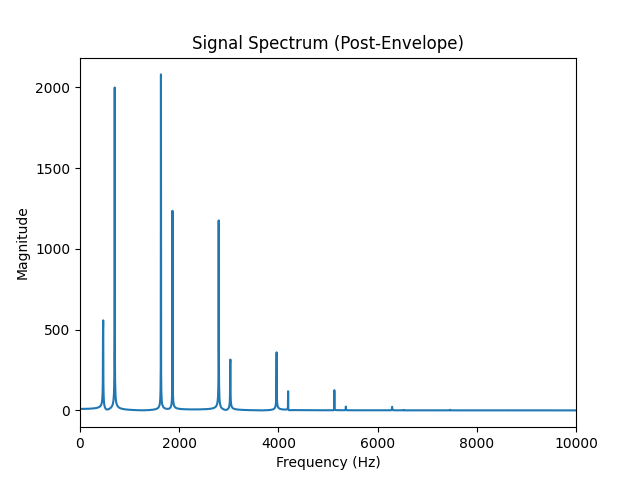
\includegraphics[width=\textwidth]{Carrier Signal Post Envelope.png}
        \caption{Carrier Signal Frequency Spectrum Post-Filter and Post-Envelope}
        \label{fig:Car post fil post env}
    \end{subfigure}
    \caption{FFT spectrum of first note of the MIDI sequence at different stages}
    \label{fig:FourImages}
\end{figure}


To model a more physical behavior of how higher pitched notes decay faster than lower pitched notes, we made our own loss function: - 

\begin{equation}
    loss\ factor = base\ loss\ factor - (pitch \ of\ note/127)*loss\ variation
\end{equation}

We defined \texttt{pickup\_ratio} and \texttt{pluck\_ratio} to input position of the pickup and the pluck position as the fraction of the total length of the left traveling buffer. This makes it easier to do the relativistic calculation according to each note of the MIDI file and its length. 

The \texttt{base\_loss\_factor} can be defined to always have certain amount of loss in energy (also defined as \texttt{loss\_factor} in the \texttt{waveGuide} class). The \texttt{loss\_variation} factor adds an additional feature to scale the overall loss factor by the pitch of the note. Higher the note, lesser is the \texttt{loss\_factor}, hence more is the loss in the energy at the bounds, hence mimicking the higher loss of higher frequencies at the bounds in real physical world. 

Another important factor to be taken into account was the duration of the note. If the note duration was lesser than the length of the buffer (calculation formula above), the output was clamped between the starting index of the note to the end index of the note. The ampplitude of the note was also taken into account by the virtue of note velocity and converting it into a scaling factor.

\begin{lstlisting}[language= Python]
start_sample = int(note.start * fs)
end_sample = int(note.end * fs)
note_duration_samples = end_sample - start_sample

amplitude = note.velocity / 127.0

# Generate audio on per note basis
note_buffer = np.zeros(note_duration_samples)
for j in range(note_duration_samples):
    note_buffer[j] = wg.wavePropagation() * amplitude

# Add to the output buffer
if start_sample + note_duration_samples <= len(output):
    output[
        start_sample : start_sample + note_duration_samples
    ] += note_buffer
\end{lstlisting}

The STFT of the output signal of waveguide synthesis shows us the sharp transients of note onsets and the dense harmonic content generated by the waveguide synthesis through its reflective delay-line interactions.

\begin{figure}[H]
    \centering
    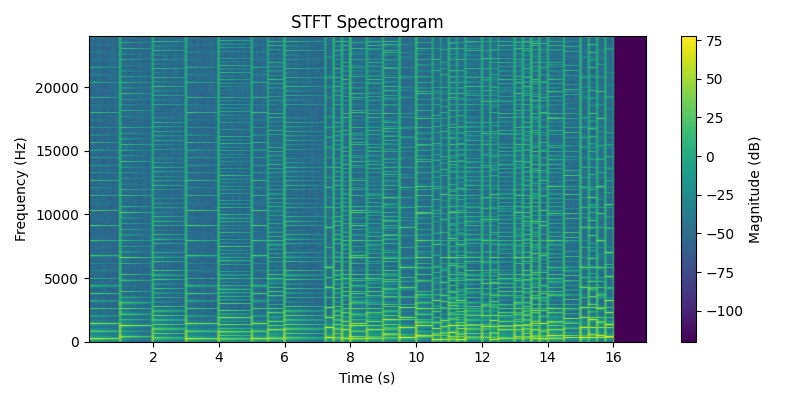
\includegraphics[width=1 \textwidth]{waveguide_spectrum.png}
    \caption{Spectrum of Physical Modeling synthesis using waveguide synthesis technique} % This is the caption that serves as the image's name
    \label{fig:waveguide spec} % This label can be used to reference the image later
\end{figure}

\subsubsection{Schroeder's reverb algorithm}

To make the sounds more natural and to make them sound as if they are coming from a natural space, we designed and implemented a reverb based on Schroeder's reverb algorithm. 

The algorithm consists of 4 arrays of gains and delay values for all pass filters arranged in series and comb filters arranged in parallel. The input signal is passed through the all-pass filter to introduce regular frequency dependent phase shifts  and the output through the all-pass filters is fed into a parallel arrangement of multiple comb filters which adds irregular phase shifts, which closely mimics real spaces. A small part of the original non-delayed signal is also mixed with the delayed signal to give a dry and wet signal balance. 

The \texttt{SchroederReverb} class that we defined accepts delay and gain arrays for all pass filters and the comb filters along with the input signal and sampling rate. 


\end{document}
